\documentclass[american,a4paper,12pt]{article}
\usepackage[T1]{fontenc} %for å bruke æøå
\usepackage[utf8]{inputenc}
\usepackage{graphicx} %for å inkludere grafikk
\usepackage{verbatim} %for å inkludere filer med tegn LaTeX ikke liker
\usepackage{mathpazo}
\usepackage{algorithm} % for algoritmene e.g paragraf 2.2 Gauss
\usepackage{algpseudocode} % lager pseudokode til algoritmene
\usepackage{amsmath}
\usepackage{caption}
\usepackage{multicol}
\usepackage{siunitx}
\usepackage{float}
\usepackage{subcaption}
\usepackage{hyperref}
\hypersetup{
    colorlinks=true,
    linkcolor=black,
    filecolor=magenta,
    urlcolor=blue,
    citecolor=blue
    pdftitle={Project 1: Computational Physics - FYS3150},
    pdfpagemode=FullScreen
}

\renewcommand{\vec}[1]{\mathbf{#1}} %ny definisjon av \vec så det blir bold face i stedet for vector-pil.

\captionsetup[table]{skip=10pt}
\bibliographystyle{plain}

\title{Project 1: Computational Physics - FYS3150}
\author{Fredrik Hoftun \& Mikkel Metzsch Jensen}
\date{September 10, 2020}
\begin{document}
\maketitle

\tableofcontents


\begin{abstract}
  The goal of this project were to... \\
  What did we do? \\
  What did we find? \\
\end{abstract}

\section{Introduction}
  In this project we will investegate different numerical approaches for the solving of the one-dimensional Poisson equation with Dirichlet boundary conditions. This is a problem that is used in many different scientiffic applications. It is used to describe electrostatic and megnetostatic phenonema in a quantitative maner. It is also helps to understand diffusion and propagation problems. The solution is generally used in a wide range of fields such as engineering, physics, mathematics, biology, chemistry, etc. \cite{poisson_paper}. In this project we have used a second derivative approximation in order to rewrite the problem as a set of linear equations. We have written three different algorithms: A general and a specialiazed algorithm using gaussian elimination and then LU demposition. Theese are described individually in the method sections along with a calculation of the number of floating point operation for each of them. Since we know the analytical solution for our problem we have compaired relative error for different choices of stepsize $h$ in the algorithm. We have also compaired of the CPU time of theese computationg. We found a significant difference in both precesion (due to round of erros) and CPU time, which are presented in the results section.

  \begin{enumerate}
    \item Motivate the reader
    \item What have I done
    \item The structure of the report
    \item conlusion?
  \end{enumerate}


\section{Method}
  \subsection{Defining the problem}
    We are going to solve the one-dimensional Poisson equation with Dirichlet boundary conditions given as the following:
    \begin{align*}
      u''(x) = f(x), \quad x \in (0,1), \quad u(0) = u(1) = 0
    \end{align*}
    In our case we will use the function:
    \begin{align*}
      f(x) = 100e^{-10x}
    \end{align*}
    Note that the algorithms for solving the problem will not be depedent on this specefic choice of f(x). The reason why we stick to this function is for the praticality of having the following analytical solution for f(x):
    \begin{align*}
      u(x) = 1 - (1 - e^{-10})x - e^{-10x}
    \end{align*}
    We can ensure that this is a valid Sslution by inserting it into the Poission equation. First we calculate double derivative of u(x):
    \begin{align*}
      u'(x) = -(1 - e^{-10}) + 10e^{-10x}, \quad u''(x) = -100e^{-10x}
    \end{align*}
    We now see that the solution satisfies the Poisson equation:
    \begin{align*}
      -u''(x) = 100e^{-10x} = f(x)
    \end{align*}
    We can therefore use this analytical solution to evaluate the precision of the numerical solutions for different choices of step length $h$.
  \subsection{Rewritting the problem as a set of linear equations}
    In order to solve the Poisson equation numerically we discretize u as $v_i$ with $n + 2$ grid points $x_i = ih$ for $i = 0, 1, \hdots, n + 1$. To clarify we have $x_0 = 0$, $x_{n+1} = 1$ which are spaced with step length $h = 1/(n + 1)$. The boundary conditions is then $v_0 = v_{n+1} = 0$. We use the following second derivative approximation
    \begin{center}
      $-u''(x_i) \approx -\frac{v_{i+1} + 2v_i - v_{i+1}}{h^2} =  f(x_i)$ \quad for $i = 1, \hdots, n$
    \end{center}
    $\Longleftrightarrow$
    \begin{align*}
      -v_{i-1} + 2v_i - v_{i+1} = h^2f(x_i)
    \end{align*}
    Notice that we cannot calculate the second derivative approximation at the end points $i = 0$ and $i = n + 1$ since we need avaliable points $v_{\pm 1}$ for the calculation. We define the colum vector $\vec{v} = [v_1, v_2, \hdots, v_n]$ and try to setup the equation for every step $i = 1, \hdots, n$. As we do this we see a usefull pattern appearing
    \begin{align*}
          \begin{bmatrix}
            2 & -1 & 0 & \cdots & 0
          \end{bmatrix}
          \begin{bmatrix}
            v_1 \\
            \vdots \\
            v_n
          \end{bmatrix}
    = h^2f(x_1)
    \end{align*}
    \begin{align*}
          \begin{bmatrix}
            2 & -1 & 0 & \cdots & \cdots & 0 \\
            -1 & 2 & -1 & 0 & \cdots & \cdots
          \end{bmatrix}
          \begin{bmatrix}
            v_1 \\
            \vdots \\
            v_n
          \end{bmatrix}
    = h^2
          \begin{bmatrix}
            f(x_1) \\
            f(x_2)
          \end{bmatrix}
    \end{align*}
    \begin{align*}
      \vdots
    \end{align*}
    \begin{align*}
          \begin{bmatrix}
            2 & -1 & 0 & \cdots & \cdots & 0 \\
            -1 & 2 & -1 & 0 & \cdots & \cdots \\
            0 & -1 & 2 & -1 & 0 & \cdots \\
            \cdots & \cdots & \cdots & \cdots & \cdots & \cdots \\
            0 & \cdots & & -1 & 2 & -1 \\
            0 & \cdots & & 0 & -1 & 2
          \end{bmatrix}
          \begin{bmatrix}
            v_1 \\
            \vdots \\
            v_n
          \end{bmatrix}
    = h^2
          \begin{bmatrix}
            f(x_1) \\
            f(x_2) \\
            \vdots \\
            f_n
          \end{bmatrix}
    \end{align*}
    \\ From this we see that we can write the problem as a linear set of equation:
    \begin{align*}
      \vec{A}\vec{v} = \vec{g}
    \end{align*}
    With the following definitions:\\
    \begin{align*}
      \vec{A} =
      \begin{bmatrix}
        2 & -1 & 0 & \cdots & \cdots & 0 \\
        -1 & 2 & -1 & 0 & \cdots & \cdots \\
        0 & -1 & 2 & -1 & 0 & \cdots \\
        \cdots & \cdots & \cdots & \cdots & \cdots & \cdots \\
        0 & \cdots & & -1 & 2 & -1 \\
        0 & \cdots & & 0 & -1 & 2
      \end{bmatrix}
      \quad, \vec{v} =
      \begin{bmatrix}
        v_1 \\
        v_2 \\
        \vdots \\
        v_n
      \end{bmatrix}
      \quad, \vec{\tilde{g}} = h^2
      \begin{bmatrix}
        f(x_1) \\
        f(x_2) \\
        \vdots \\
        f_n
      \end{bmatrix}
    \end{align*}
\subsection{General solution using Gausian elimination}
We can solve our set of linear equations using Gaussian elimination on the matrix $\vec{A}\vec{v} = \vec{g}$. In the beginning we assume a more generilazed matrix $\vec(A)$ as:
\begin{align*}
  A =
  \begin{bmatrix}
    b_1 & c_1 & 0 & \cdots & \cdots & 0 \\
    a_1 & b_2 & c_2 & 0 & \cdots & \cdots \\
    0 & a_2 & b_3 & c_3 & 0 & \cdots \\
    \cdots & \cdots & \cdots & \cdots & \cdots & \cdots \\
    0 & \cdots & & a_{n-2} & b_{n-1} & c_{n-1} \\
    0 & \cdots & & 0 & a_{n-1} & b_n
  \end{bmatrix}
\end{align*}
\\ Here $a_i$ are the elements below the diagonal, $b_i$ are the elements on the diagonal and $c_i$ are the elements above the diagonal. In order to solve this we use first a forward substitution and then a backwards substitution \cite{linalg}. The implementation of this is showed in Algorithm 1:
\begin{algorithm}[H]
\caption{General algorithm}
\begin{algorithmic}[1] %fra algpseudocode
  \For {$i = 2, \dots, n$} \Comment{Forward substitution eliminating $a_i$}
    \State $b_i = b_i - c_{i-1}\cdot {a_i}/{{b}_{i-1}}$ \Comment{Update ${b}_i$}
    \State $g_i = g_i - {g}_{i-1}\cdot {a_i}/{{b}_{i-1}}$ \Comment{Update ${g}_i$}
  \EndFor
  \Statex
  \State $v_0 = v_{n+1} = 0$ \Comment{Backward substitution obtaining $v_i$}
  \State $v_n = g_n/B_n;$
  \For {$i = n-1, \dots, 1$}
    \State $v_i = (g_i - c_i\cdot v_{i+1})/b_i$ % \frac{g_i - c_i\cdot v_{i+1}}{b_i}$
  \EndFor
\end{algorithmic}
\end{algorithm}
By running this algorithm for decreasing step length we se that the numerical solution aproaches the analytical quite fast (see figure \ref{fig:general_ex})
\begin{figure}[H]
\begin{center}
  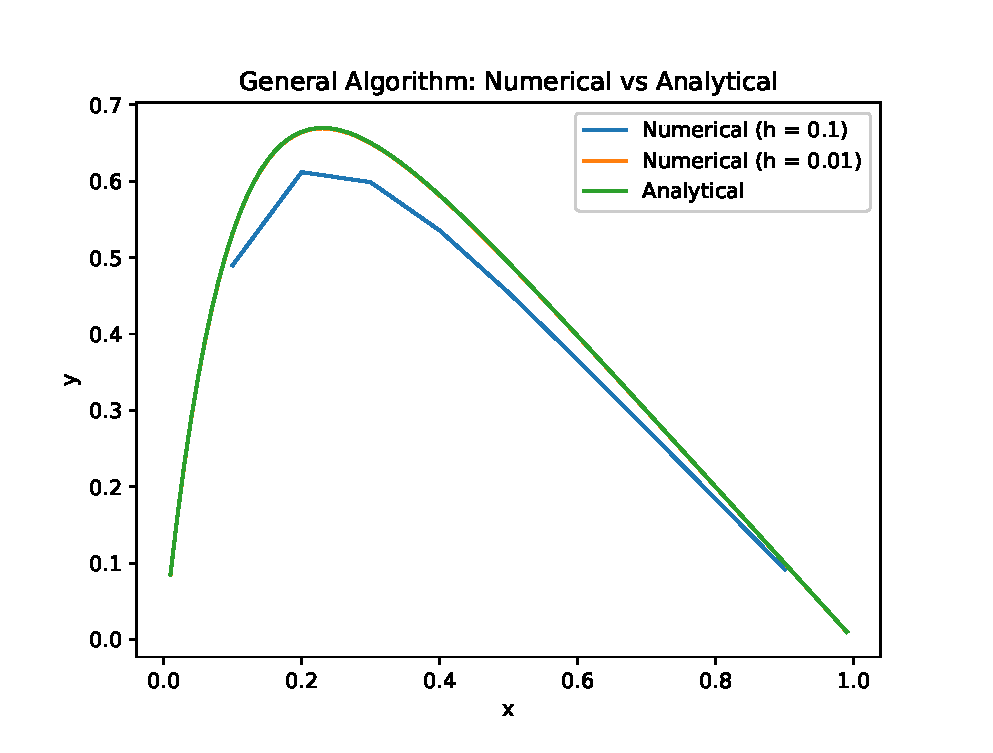
\includegraphics[width = \textwidth]{figures/general_algo_example.eps} \\
  \caption{The figure shows the analytical solution and the numerical solution using the generel algorithm for $h = 0.1$ and $h = 0.01$ respectively. We see that the numerical solution lines up with the analytical solution already for $h = 0.01$.}
  \label{fig:general_ex}
  \end{center}
\end{figure}
We can calculate the algorithms number of Floating Point Operations. In our forward substitution we have $2 \cdot 3$ operations for each loop which runs for a total of n-1 times. In the backward substitution we have a single leading operation and then 3 operations which loops for a total of n-1. The total number of operations is then
\begin{align*}
  (6 + 3)(n - 1) + 1 = 9n - 8
\end{align*}
For large n we can approximate this as 9n.
\subsection{Simplified specific solution}
Since we have fixed value $a = -1,\ b = 2,\ c = -1$ for the matrix A introduced in previous section, we can simplify our algorithm even more. Now we can do the forward substitution before hand:
 $\vec{A}$:
\begin{align*}
    \vec{A} =
    \begin{bmatrix}
    2 & -1 & 0 & \cdots & \cdots & 0 \\
    -1 & 2 & -1 & 0 & \cdots & \cdots \\
    0 & -1 & 2 & -1 & 0 & \cdots \\
    \cdots & \cdots & \cdots & \cdots & \cdots & \cdots \\
    0 & \cdots & & -1 & 2 & -1 \\
    0 & \cdots & & 0 & -1 & 2
    \end{bmatrix}
    \ \sim \
    \begin{bmatrix}
    2 & -1 & 0 & \cdots & \cdots & 0 \\
    0 & 3/2 & -1 & 0 & \cdots & \cdots \\
    0 & -1 & 2 & -1 & 0 & \cdots \\
    \cdots & \cdots & \cdots & \cdots & \cdots & \cdots \\
    0 & \cdots & & -1 & 2 & -1 \\
    0 & \cdots & & 0 & -1 & 2
    \end{bmatrix}
\end{align*}
\begin{align*}
    \quad \sim
    \begin{bmatrix}
    2 & -1 & 0 & \cdots & \cdots & 0 \\
    0 & 3/2 & -1 & 0 & \cdots & \cdots \\
    0 & 0 & 4/3 & -1 & 0 & \cdots \\
    \cdots & \cdots & \cdots & \cdots & \cdots & \cdots \\
    0 & \cdots & & -1 & 2 & -1 \\
    0 & \cdots & & 0 & -1 & 2
    \end{bmatrix}
    \ \sim \
    \begin{bmatrix}
    2 & -1 & 0 & \cdots & \cdots & 0 \\
    0 & 3/2 & -1 & 0 & \cdots & \cdots \\
    0 & 0 & 4/3 & -1 & 0 & \cdots \\
    \cdots & \cdots & \cdots & \cdots & \cdots & \cdots \\
    0 & \cdots & & 0 & i_n/{i_n-1} & -1 \\
    0 & \cdots & & 0 & 0 & {i_n+1}/i_n
    \end{bmatrix} \\
\end{align*}
We see that the updated diagonal element $b_i$ follows the formula:
\begin{align*}
   b_i = \frac{i+1}{i}
\end{align*}
This means that the update of the diagonal element now use 2 floating point operations per n in where the general one used 3 per n. But the most important fact is that this can be precalculated and in practice excluded from the algorithm. We can therefore justify not to count theese floating point operations. The update of $g_i$ with known values for a, b and c simplifies to:
\begin{align*}
  g_i = g_i + g_{i-1}/{b_{i-1}}
\end{align*}
\cite{linalg}. This gives us the following simplified algorithm:
\begin{algorithm}[H]
\caption{Special algorithm, where $a_i = -1,\ b_i = 2,\ c_i = -1$}
\begin{algorithmic}[1]
  \For {$i = 2, \dots, n$} \Comment{Forward substitution eliminating $a_i$}
    \State $b_i = {i+1}/i$ \Comment{Update ${b}_i$}
    \State $g_i = g_i + g_{i-1}/{b_{i-1}}$ \Comment{Update $g_i$}
  \EndFor
  \Statex
  \State $v_n = 0$ \Comment{Backward substitution obtaining $v_i$}
  \For {$i = n-1, \dots, 1$}
    \State $v_i = \frac{g_i + v_{i+1}}{b_i}$
  \EndFor
\end{algorithmic}
\end{algorithm}
Similarly to the general algorithm we can calculate total number of floating point operations (not including calculation of $b_i$):
\begin{align*}
  (2 + 2)(n-2) = 4n - 8
\end{align*}
For large n this can be approximated to $4n$.
\\
PLOT OR EXAMPLE OF CODE WORKING?
\subsection{LU decomposition}
For the LU decomposition we have our triangular matrix $\vec{A}$ which can be divided into two invertible matrices, consisting of one upper triangular matrix $\vec{U}$ and one lower triangular matrix $\vec{L}$. We then get the LU decomposition:
\begin{align*}
    \vec{Av} &= \vec{g} = \vec{LUv}\\
    \vec{Uv} &= \vec{L^{-1}g = \vec{w}}
\end{align*}
The Armadillo library for \verb!C++! allows for easy computation of the matrices.\\
Her kommer noe om FLOPS

\subsubsection*{Proof that L or U is invertible}
A matrix is invertible if the determinant is not equal to zero; $\det A \neq 0$. A property of triangular matrices is that the determinant is the product of the values on the diagonal. In our case we have non-zero real numbers so the matrices are invertible.

\subsection{Comparing precision and time}
In order to compare the precesion of the different solutions we will use the relative error between the numerical solution ($v_i$) and the analytical solution (($f(x_i)$). For practical reasons we will use the take the logarithm (base 10) so the relative error is given as
\begin{align*}
  \epsilon_i = log_{10}\left|\frac{v_i - u_i}{u_i}\right|
\end{align*}
Since we divide with the analytical solution $u_i$ we cannot make this calculation for the end points where $u_0 = u_{n+1} = 0$. This means that we will calculate $\epsilon_i$ for $i 1, \hdots, n$. When we lower the step length $h$ we expect the error to decrease as well. When plotting $h$ with a logaritmic axis (base 10) against $\epsilon_i$ we should see a linear trend. The slope of this trend can then be usefull in order determain the relationship between precesion and step length. At some point though we could expiernce that this trend is interrupted by erros in floating-point arithmetic due to round-off. We want to investegate if and when this happens.\\
In addition to the precesion comparing we will also investegate whether we see any different in CPU time between the different algorithms. This should reflect back on the number of floating point operations done in each of them.
\subsection{Implementation}
We used \verb!C++! to implement our algorithms. The results are then written to a text file and read by a python script for the presentation of the results.

\section{Results}
  GITHUB LINK HERE \\
  We collected the max of the relative error $\epsilon$ for different values of the step length $h$ for all the three algorithms. The result is shown in figure \ref{fig_max_err}
  \begin{figure}[H]
  \begin{center}
    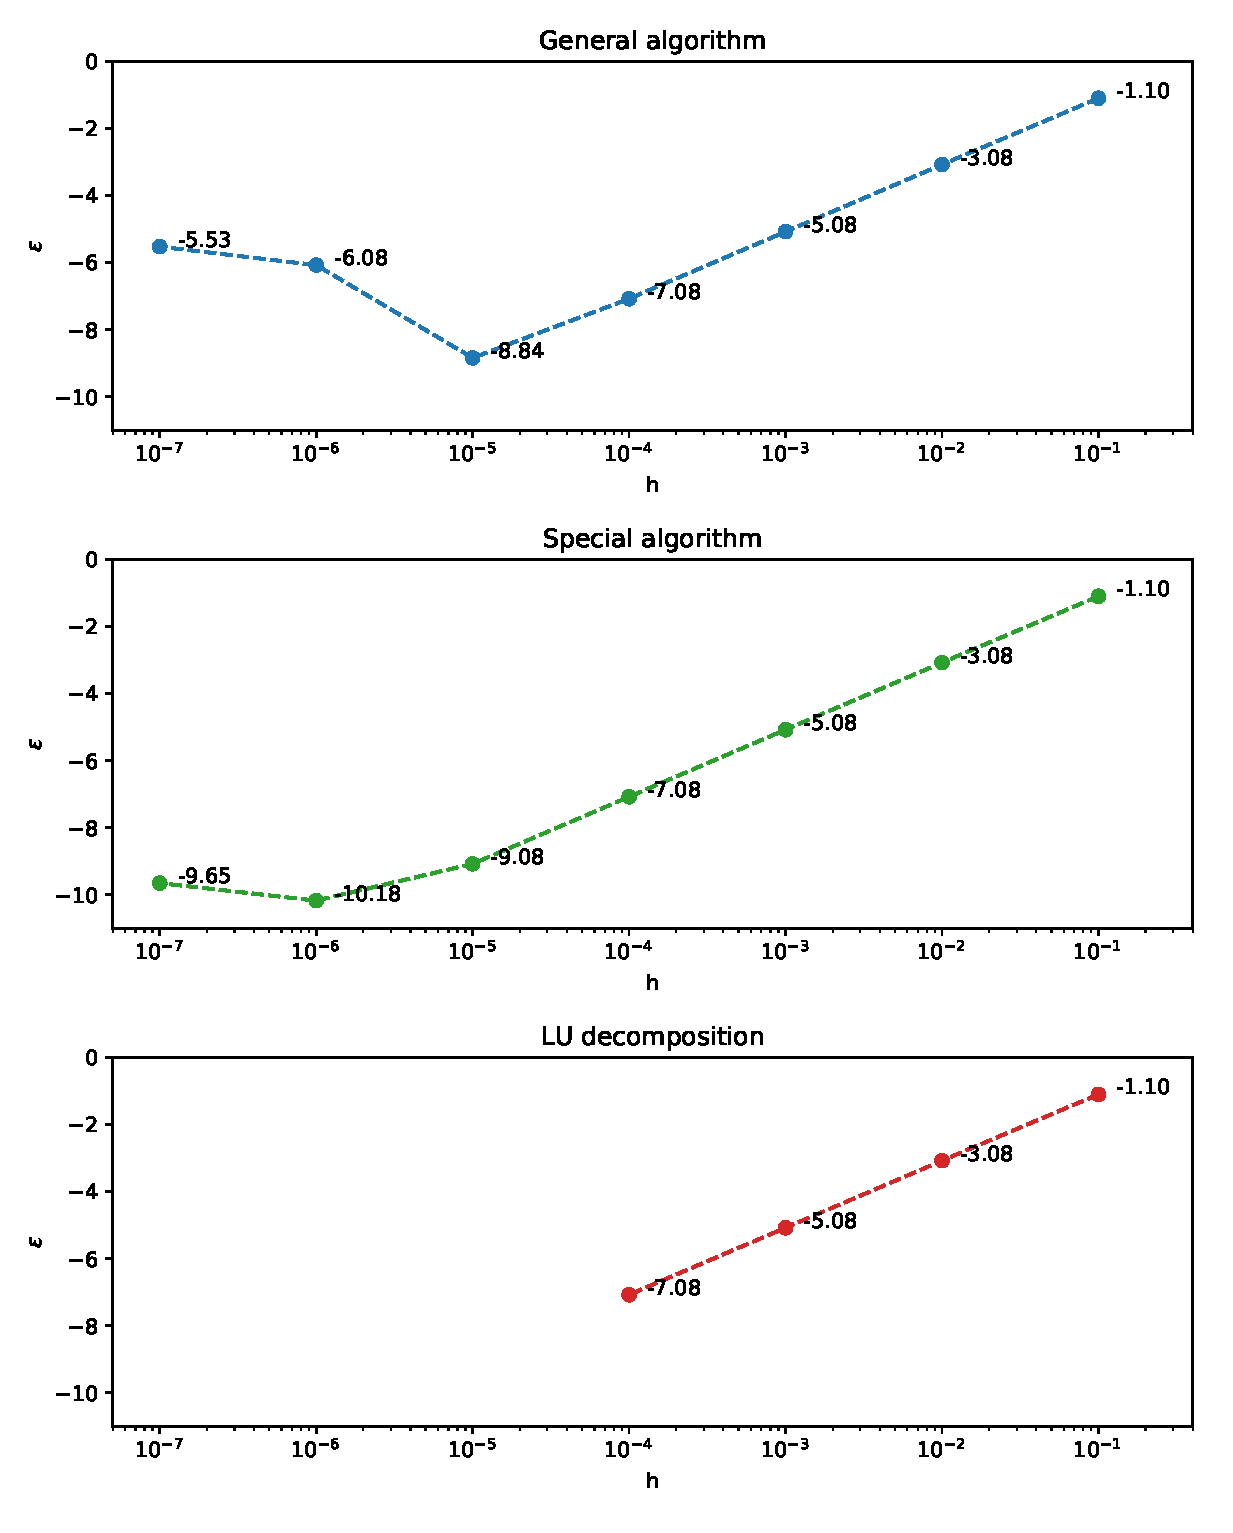
\includegraphics[width = \textwidth]{figures/max_err.eps} \\
    \caption{Relative error $\epsilon$ for different step length $h$. The relative error is defined with a logarithm and h is plotted on a logaritmic axis.}
    \label{fig:max_err}
    \end{center}
  \end{figure}
  Note that we were not able to produce the results for LU decompositions with $h \le \num{e-5}$ meaning that we could not store a matrix of size $\num{e5} \times \num{e5}$ or larger. \\
  The CPU time for the execution of the different runs can be seen in table \ref{tab:final_res}. Note that this varied a lot between each repetition of measurements
  \begin{table}[H]
    \begin{center}
    \caption{CPU Time}
    \begin{tabular}{|c|c|c|c|} \hline
    \textbf{N} & \textbf{General algorithm: t [s]} & \textbf{Special algorithm: t [s]} & \textbf{LU Decomposition: t [s]} \\ \hline
    $10^1$ & $\num{3e-6}$     & $\num{3e-6}$    & $\num{9.81e-4}$ \\ \hline
    $10^2$ & $\num{4e-6}$     & $\num{4e-6}$    & $\num{1.96e-4}$ \\ \hline
    $10^3$ & $\num{3.8e-5}$   & $\num{3.7e-5}$  & $\num{1.02e-2}$ \\ \hline
    $10^4$ & $\num{3.41e-4}$  & $\num{3.54e-4}$ & $\num{2.45e0}$ \\ \hline
    $10^5$ & $\num{3.79e-3}$  & $\num{3.50e-3}$ & nan \\ \hline
    $10^6$ & $\num{3.57e-2}$  & $\num{3.24e-2}$ & nan \\ \hline
    $10^7$ & $\num{3.16e-1}$  & $\num{3.24e-1}$ & nan \\ \hline
    \end{tabular}
    \end{center}
    \label{tab:final_res}
  \end{table}
  The computer which we run all the programs on have the following CPU specs:
  \begin{center}
    CPU = 2.5 GHz Intel Core i5
  \end{center}
\section{Discussion}
Regarding the development of the maximum relative error (show in figure \ref{fig:max_err}) we archived the expected trend that we were looking for. For all the algorithms we get a linear connection between $h$ and $\epsilon$ for $h \ge \num{e-4}$. For this section see that $\epsilon$ drops about 2 points for each logarithmic decreasement in h. This tell us that the error is proportional to $h^2$:
\begin{align*}
  \epsilon = \mathcal{O}(h^2)
\end{align*}
From the results we also see that the linear trend is broken at some point given us a point of minimum error. Since we were not able to go lower than $h = \num{-4}$ for the LU decomposition we can only compare the general and special algorithm here. In this case we see in both cases that the linear trend is broken around $h = \num{-5}$. For the general algorithm this happens quite drastically leavning us with a minimum (maximum) relative error of -8.84. For the special algorithm the error keeps decreasing all the way down to -10.18 at $h = \num{-6}$. This loss of precision happens due to round-off erros when handling to small increaments $h$. In the case of the special algorithm we see that the simplified calculations make us able to archieve higher precesion. Not only is this more efficient in relation to computer processing needed but also in maximum precesion that are able to archive. If we had to extract the most reliable solution from this problem we should choose the special algorithm with $h = \num{-6}$. Note that this might not be the precise minimum point, and we could still very $h$ in even smaller increaments to check for lower relative error. \\
Regarding the CPU time we got some mixed results. Waiting to see if FREDRIK fixes better data. 




The computer should be able to make a maximum of $\num2.5e9$ floating point operations pr. second. We can inevestegate the number of FLOPS for the general algorithm with $n = \num{e7}$:
\begin{center}
  $FP = \num{9e7} - 17 \approx \num{9e7}$
\end{center}
\begin{center}
  $\text{CPU Time} = 0.316 \ s$
\end{center}
\begin{center}
  FLOPS = FP / CPU Time $\approx 0.28 \ GHz$
\end{center}
We see that there are some room up the maximum capacity of the processor (2.5 GHz), but this might be somewhat expectable

\section{Conclusion}
In this report we have used three different ways of computing $\vec{A}\vec{v} = \vec{g}$ and have seen that efficiency of the methods vary greatly. We have witnessed the importance of efficient implementation of algorithms ...


\begin{thebibliography}{9}
  \bibitem{poisson_paper} S. B. Gueye, K. Talla and C. Mbow, "Solution of 1d poisson equation with neumann-dirichlet and dirichlet-neumann boundary conditions using the finite difference method", Journal of Electromagnetic Analysis and Applications, Vol. 6, No. 10, pp. 309, 2014.

  \bibitem{linalg} Hjort-Jensen, M., 2018. Computational Physics Lectures: Linear Algebra methods,  accesable at course github repository. \url{http://compphysics.github.io/ComputationalPhysics/doc/pub/linalg/pdf/linalg-print.pdf}







\end{thebibliography}

\end{document}
